%% Numerical Experiment Report Template %%
%----------------------------------------------------%
\documentclass[a4paper,11pt]{article}

%---------------code settings------------------------%
\usepackage{listings}
\usepackage{xcolor}
\definecolor{mygreen}{rgb}{0,0.6,0}
\definecolor{mygray}{rgb}{0.5,0.5,0.5}
\definecolor{mymauve}{rgb}{0.58,0,0.82}

\lstset{ %
  backgroundcolor=\color{white},   % choose the background color; you must add \usepackage{color} or \usepackage{xcolor}
  basicstyle=\footnotesize,        % the size of the fonts that are used for the code
  breakatwhitespace=false,         % sets if automatic breaks should only happen at whitespace
  breaklines=true,                 % sets automatic line breaking
  captionpos=bl,                    % sets the caption-position to bottom
  commentstyle=\color{mygreen},    % comment style
  deletekeywords={...},            % if you want to delete keywords from the given language
  escapeinside={\%*}{*)},          % if you want to add LaTeX within your code
  extendedchars=true,              % lets you use non-ASCII characters; for 8-bits encodings only, does not work with UTF-8
  frame=single,                    % adds a frame around the code
  keepspaces=true,                 % keeps spaces in text, useful for keeping indentation of code (possibly needs columns=flexible)
  keywordstyle=\color{blue},       % keyword style
  %language=Python,                 % the language of the code
  morekeywords={*,...},            % if you want to add more keywords to the set
  numbers=left,                    % where to put the line-numbers; possible values are (none, left, right)
  numbersep=5pt,                   % how far the line-numbers are from the code
  numberstyle=\tiny\color{mygray}, % the style that is used for the line-numbers
  rulecolor=\color{black},         % if not set, the frame-color may be changed on line-breaks within not-black text (e.g. comments (green here))
  showspaces=false,                % show spaces everywhere adding particular underscores; it overrides 'showstringspaces'
  showstringspaces=false,          % underline spaces within strings only
  showtabs=false,                  % show tabs within strings adding particular underscores
  stepnumber=1,                    % the step between two line-numbers. If it's 1, each line will be numbered
  stringstyle=\color{orange},     % string literal style
  tabsize=2,                       % sets default tabsize to 2 spaces
  %title=myPython.py                   % show the filename of files included with \lstinputlisting; also try caption instead of title
}

%---------------------other package--------------&
\usepackage[T1]{fontenc}
\usepackage[utf8x]{inputenc}
\usepackage[english]{babel}
\usepackage{float}
\usepackage[colorlinks=true, allcolors=blue]{hyperref}
\usepackage[parfill]{parskip}
\usepackage[a4paper,top=2cm,bottom=3cm,left=1.5cm,right=1.5cm,marginparwidth=2cm]{geometry}
\usepackage{graphicx}
\usepackage{fancyhdr}
\usepackage{titlesec}
\usepackage{amsmath}
\usepackage{indentfirst}
\setlength{\headheight}{30pt}
\setlength{\parindent}{2em}


\begin{document}

%--------------fancyhead------------%
\pagestyle{fancy}
\fancyhead[R]{Numerical Experiment B}
\fancyhead[L]{
\includegraphics[width=4.5cm]{logo/row.png}}
\fancyfoot[R]{
\includegraphics[width=3cm]{logo/spst.png}}
%---------------title---------------%
\title{\textbf{\Huge{Numerical Experiment B}}}

%--------------author---------------%
\author{\textit{Xinzhi Li} \\\quad\\Student ID:~~$\boldsymbol{2022211084}$\\\quad\\ \textit{School of Physics Science and Technology, ShanghaiTech University, Shanghai 201210, China}\\\quad \\ \textit{Email address}:\quad lixzh2022@shanghaitech.edu.cn}



%---------------Logo----------------%
\begin{figure*}[t]
\centering

\includegraphics[width=1\columnwidth]{logo/row.png}
\end{figure*}

%--------------maketitle--------------&
\maketitle\thispagestyle{empty}

%------------titlesection-------------%
\titleformat{\section}[block]{\large \bfseries}{\Roman{section}.}{1em}{\centering\MakeUppercase}[]
\titlespacing{\section}{2pt}{16pt}{10pt}
\titleformat{\subsection}[block]{}{\Alph{subsection}.}{1em}{\centering}
\titlespacing{\subsection}{2pt}{8pt}{4pt}
%--------------main body--------------&
\newpage
\setcounter{page}{1}
\section{Introducion}
\textit{\textbf{Interpolation}} and \textit{\textbf{Iteration}} are the most common numerical methods. The former is a type of estimation, a method of constructing new data points based on the range of a discrete set of known data points in the mathematical field of numerical analysis. The latter is the repetition of a process in order to generate a sequence of outcomes which can produce approximate numerical solutions to some certain problems. In engineering and science, one often has a number of data points, obtained by sampling or experimentation, which represent the values of a function for a limited number of values of the independent variable. It is often required to interpolate; that is, estimate the value of that function for an intermediate value of the independent variable. We will use some interpolation methods to approximate functions and use \textit{\textbf{Newton's iteration}} to solve nonlinear equations.

\section{Problem}
\begin{enumerate}
    \item Use \textit{\textbf{Lagrange interpolating polynomial}} to approximate the function 
    \begin{eqnarray}
        f(x)=\dfrac{1}{1+25x^2}\quad\quad\quad\quad x\in[-1,1]
    \end{eqnarray}
    and observe the Runge phenomenon.
    \item The population of China from 1988 to 1996 is given by:
    \begin{table}[h]
        \centering
        \begin{tabular}{c|c|c|c|c|c|c|c|c|c}
            \hline
            & & & & & & & & &\\[-6pt]
            year&1988&1989&1990&1991&1992&1993&1994&1995&1996\\
            \hline
            & & & & & & & & &\\[-6pt]
            population($\times 10^{8}$)&11.10&11.27&11.43&11.58&11.72&11.85&11.99&12.11&12.24\\
            \hline
        \end{tabular}
        \caption{The population from 1988 to 1996}
    \end{table}
    
    According to the data above and predict the population in 2018, 2019. Use \textit{\textbf{Malthusian growth model}}, 
    \begin{eqnarray}
        N(t)=e^{a+bt}
    \end{eqnarray}
    where $N(t)$ is the number of population. Take logarithm,
    \begin{eqnarray}
        \textrm{ln}N(t)=y(t)=a+bt
    \end{eqnarray}
    
    \item Given nonlinear equations
    \begin{eqnarray}
        F(x)=\begin{cases}
            3x_1-\cos(x_2x_3)-\dfrac{1}{2}=0\\
            ~\\
            x_1^2-81(x_2+0.1)+\sin x_3+1.06=0\\
            ~\\
            e^{-x_1x_2}+20x_3+\dfrac{1}{3}(10\pi-3)=0
        \end{cases}
    \end{eqnarray}
    Use \textit{\textbf{Newton's iteration}} to solve the equations with $\epsilon=10^{-5}$. Calculate the iterations.
\end{enumerate}

\section{Numerical Results}
\begin{enumerate}
    \item We take $n$ nodes:$-1\leq x_1<x_2\dotsm<x_n\leq 1$, the lagrange interpolating polynomial is given by
    \begin{eqnarray}
        l_{k}(x)=\prod_{j\neq k}\dfrac{x-x_j}{x_k-x_j}
    \end{eqnarray}
    Then the approximated function is 
    \begin{eqnarray}
        L=\sum_{k=1}^{n}l_{k}(x)f(x_k)
    \end{eqnarray}
    The results are shown in Figure~\ref{fig1}
    \begin{figure}[h]
        \centering
        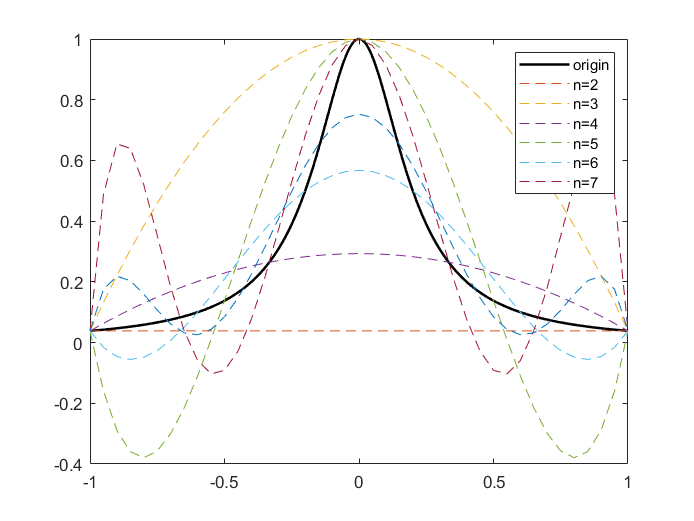
\includegraphics[width=0.3\textwidth]{1.png}
        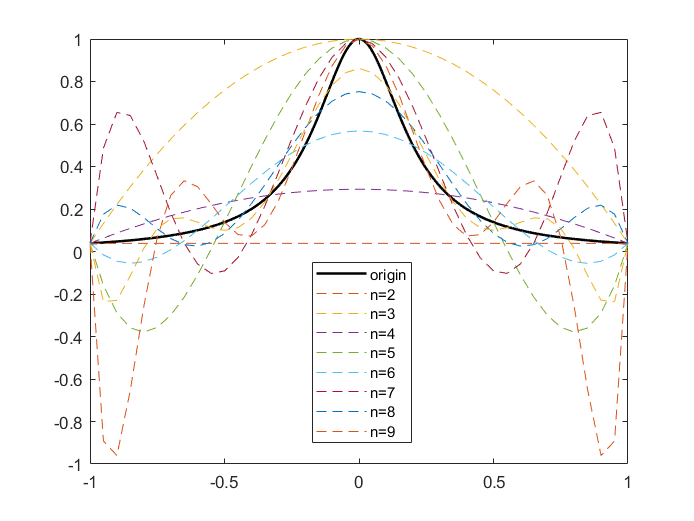
\includegraphics[width=0.3\textwidth]{2.png}
        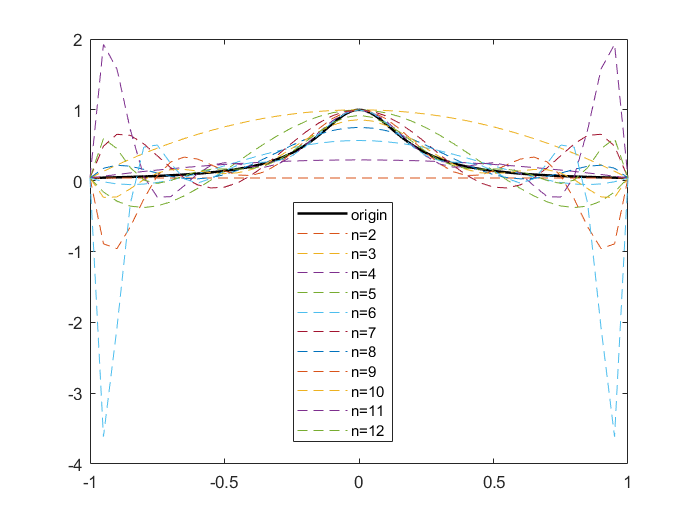
\includegraphics[width=0.3\textwidth]{3.png}\caption{Lagrange interpolating polynomial}
        \label{fig1}
    \end{figure} 

    \item We use least square to fix the curve, the resulting function is shown in Figure~\ref{fig2}
    \begin{figure}[h]
        \centering
        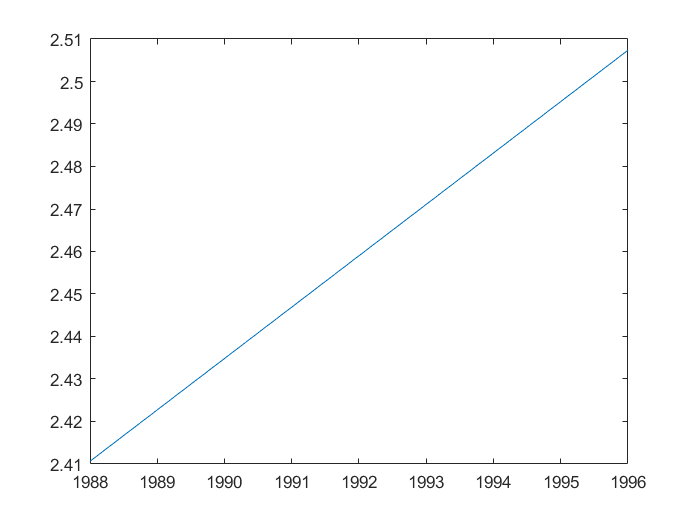
\includegraphics[width=0.3\textwidth]{4.png}\\
        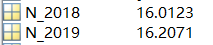
\includegraphics[width=0.2\textwidth]{5.png}\caption{}
        \label{fig2}
    \end{figure}

    \item The Newton's iteration is given by 
    \begin{eqnarray}
        x^{(k+1)}=x^{(k)}-[\nabla F(x^{(k)})]^{-1}F(x^{(k)}),\quad\quad k=0,1,2,\dotsm
    \end{eqnarray}
    where
    \begin{eqnarray}
        \nabla F = \begin{pmatrix}
            \dfrac{\partial f_1}{\partial x_1}&\dfrac{\partial f_1}{\partial x_2}&\dotsm&\dfrac{\partial f_1}{\partial x_n}\\
            \dfrac{\partial f_2}{\partial x_1}&\dfrac{\partial f_2}{\partial x_2}&\dotsm&\dfrac{\partial f_2}{\partial x_n}\\
            &&\dotsm&\\
            \dfrac{\partial f_n}{\partial x_1}&\dfrac{\partial f_n}{\partial x_2}&\dotsm&\dfrac{\partial f_n}{\partial x_n}\\
        \end{pmatrix}
    \end{eqnarray}

    We start with $x^{(0)}=(0,0,0)^T$. Then the total iteration is 3, and the solution is
    \begin{eqnarray}
        x=\begin{pmatrix}
            0.4996\\
            -0.0900\\
            -0.5259\\
        \end{pmatrix}
    \end{eqnarray}
\end{enumerate}

\section{Remark}
We have observed the Runge phenomenon, that is, with the increasing nodes and the dimension of the polynomials, it becomes more accurate, but after $n=7$, the result performs a large deviation at the either end. The best approximation depends on the interval that you want.

According to the data in 2018 and 2019, the population is $1.405\times 10^{9}$ and $1.410\times 10^{9}$. It perhaps due to the lifestyle is totally changed for the young generation and the marriage rate decreases. 

The Newton's iteration is so fast, since it is a quadratic approach algorithm.
\section{Code}
\lstinputlisting{lagrange.m}
\lstinputlisting{population.m}
\lstinputlisting{Newton.m}

\end{document}